\documentclass[aspectratio=169]{beamer}
\useoutertheme[progressbar=frametitle]{metropolis}
\useinnertheme{metropolis}
\definecolor{nabgray}{rgb}{0.6,0.59,0.61}
\usecolortheme[named=nabgray]{structure}

\usepackage{tikz}
\usepackage[utf8]{inputenc}
\usepackage[spanish]{babel}
\usepackage{fontspec}
\usepackage{ulem}

\setmonofont{JetBrains Mono}
\setmainfont{Roboto}
\setsansfont{Roboto}


\usepackage{smartdiagram}
\usepackage{qtree}
\usepackage{verbatim}
\usepackage{svg}
\usepackage{graphicx}
\usepackage{color}


\definecolor{lightgray}{rgb}{0.95, 0.95, 0.95}
\definecolor{darkgray}{rgb}{0.4, 0.4, 0.4}
%\definecolor{purple}{rgb}{0.65, 0.12, 0.82}
\definecolor{editorGray}{rgb}{0.95, 0.95, 0.95}
\definecolor{editorOcher}{rgb}{1, 0.5, 0} % #FF7F00 -> rgb(239, 169, 0)
\definecolor{editorGreen}{rgb}{0, 0.5, 0} % #007C00 -> rgb(0, 124, 0)
\definecolor{orange}{rgb}{1,0.45,0.13}
\definecolor{olive}{rgb}{0.17,0.59,0.20}
\definecolor{brown}{rgb}{0.69,0.31,0.31}
\definecolor{purple}{rgb}{0.38,0.18,0.81}
\definecolor{lightblue}{rgb}{0.1,0.57,0.7}
\definecolor{lightred}{rgb}{1,0.4,0.5}
\definecolor{ocherCode}{rgb}{1, 0.5, 0} % #FF7F00 -> rgb(239, 169, 0)
\definecolor{blueCode}{rgb}{0, 0, 0.93} % #0000EE -> rgb(0, 0, 238)
\definecolor{greenCode}{rgb}{0, 0.6, 0} % #009900 -> rgb(0, 153, 0)


\usepackage{upquote}
\usepackage{listings}
\lstdefinelanguage{JavaScript}{
    morekeywords=[1]{break, continue, delete, else, for, function, if, in,
        new, return, this, typeof, var, void, while, with},
    % Literals, primitive types, and reference types.
    morekeywords=[2]{false, null, true, boolean, number, undefined,
        Array, Boolean, Date, Math, Number, String, Object},
    % Built-ins.
    morekeywords=[3]{eval, parseInt, parseFloat, escape, unescape},
    % Basic design
    backgroundcolor=\color{lightgray},
    basicstyle={\small\ttfamily},
    frame=l,
    keywordstyle=\footnotesize\color{blue},
    escapeinside={<@}{@>},
    breaklines=true,
    % Line numbers
    xleftmargin={0.75cm},
    numbers=left,
    stepnumber=1,
    firstnumber=1,
    numberfirstline=true
    % Code design
    identifierstyle=\color{black},
    keywordstyle=\color{ocherCode}\bfseries,
    ndkeywordstyle=\color{greenCode}\bfseries,
    stringstyle=\color{ocherCode}\ttfamily,
    commentstyle=\color{darkgray}\ttfamily,
    tabsize=2,
    showtabs=true,
    showspaces=false,
    showstringspaces=false,
    extendedchars=true,
    breaklines=true
}[keywords, comments, strings]

\colorlet{punct}{red!60!black}
\definecolor{background}{HTML}{EEEEEE}
\definecolor{delim}{RGB}{20,105,176}
\colorlet{numb}{magenta!60!black}

\lstdefinelanguage{json}{
    basicstyle=\normalfont\ttfamily,
    numbers=left,
    numberstyle=\scriptsize,
    stepnumber=1,
    numbersep=8pt,
    showstringspaces=false,
    breaklines=true,
    frame=lines,
    literate=
    *{0}{{{\color{numb}0}}}{1}
    {1}{{{\color{numb}1}}}{1}
    {2}{{{\color{numb}2}}}{1}
    {3}{{{\color{numb}3}}}{1}
    {4}{{{\color{numb}4}}}{1}
    {5}{{{\color{numb}5}}}{1}
    {6}{{{\color{numb}6}}}{1}
    {7}{{{\color{numb}7}}}{1}
    {8}{{{\color{numb}8}}}{1}
    {9}{{{\color{numb}9}}}{1}
    {:}{{{\color{punct}{:}}}}{1}
    {,}{{{\color{punct}{,}}}}{1}
    {\{}{{{\color{delim}{\{}}}}{1}
    {\}}{{{\color{delim}{\}}}}}{1}
    {[}{{{\color{delim}{[}}}}{1}
    {]}{{{\color{delim}{]}}}}{1},
}
\lstset{language=java,
	otherkeywords={var,record},
	% Basic design
	backgroundcolor=\color{lightgray},
	basicstyle={\small\ttfamily},
	frame=l,
	keywordstyle=\footnotesize\color{blue},
	escapeinside={<@}{@>},
	breaklines=true,
	% Line numbers
	xleftmargin={0.75cm},
	numbers=left,
	stepnumber=1,
	firstnumber=1,
	numberfirstline=true
	% Code design
	identifierstyle=\color{black},
	keywordstyle=\color{ocherCode}\bfseries,
	ndkeywordstyle=\color{greenCode}\bfseries,
	stringstyle=\color{ocherCode}\ttfamily,
	commentstyle=\color{darkgray}\ttfamily,
	tabsize=2,
	showtabs=true,
	showspaces=false,
	showstringspaces=false,
	extendedchars=true,
	breaklines=true
}


\usebackgroundtemplate%
{%
    
\includegraphics[width=\paperwidth]{Images/Contenido}%
}

\definecolor{celeste}{HTML}{5E91AA}
\definecolor{azul}{HTML}{163F54}

\setbeamercolor{head1}{fg=celeste}
\setbeamercolor{title}{fg=celeste}
\setbeamercolor{subtitle}{fg=celeste}
\setbeamercolor{frametitle}{fg=celeste}
\setbeamercolor{structure}{fg=azul}
\setbeamercolor{normal text}{fg=azul}


\title{Java y su ecosistema}
\author{Víctor Orozco}
\institute{}
\date{\today}

\begin{document}

\frame{\titlepage}

\section{Intro}



\begin{frame}{Principios de sobrevivencia - Redmonk}
	\begin{figure}
		\centering
		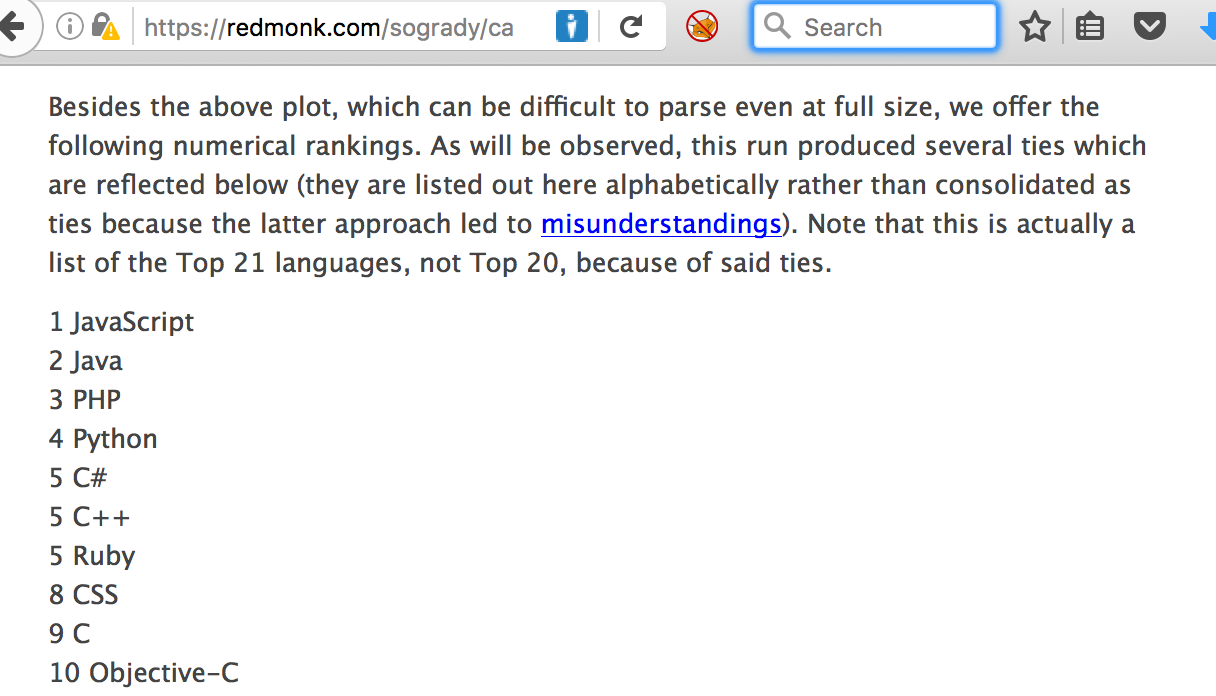
\includegraphics[width=0.7\linewidth]{Images/redmonk}
	\end{figure}
\end{frame}

\begin{frame}{Principios de sobrevivencia - Tiobe}
	\begin{figure}
		\centering
		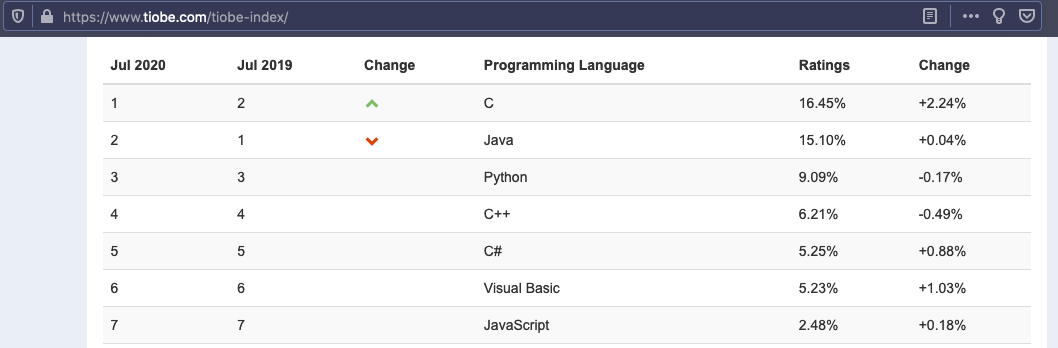
\includegraphics[width=0.9\linewidth]{Images/tiobe}
	\end{figure}
\end{frame}

\begin{frame}{Principios de sobrevivencia - IEEE}
	\begin{figure}
		\centering
		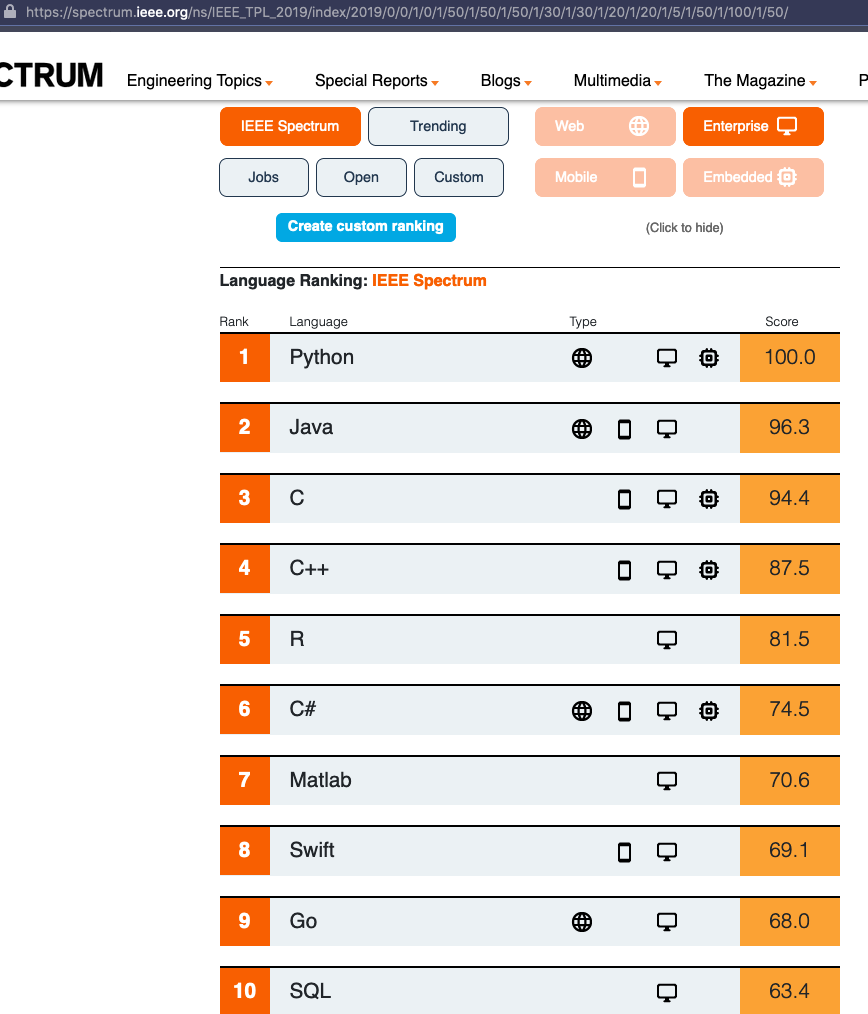
\includegraphics[width=0.8\linewidth]{Images/ieeeenterpise}
	\end{figure}
\end{frame}

\begin{frame}{Principios de sobrevivencia - Forbes}
    \begin{figure}
        \centering
        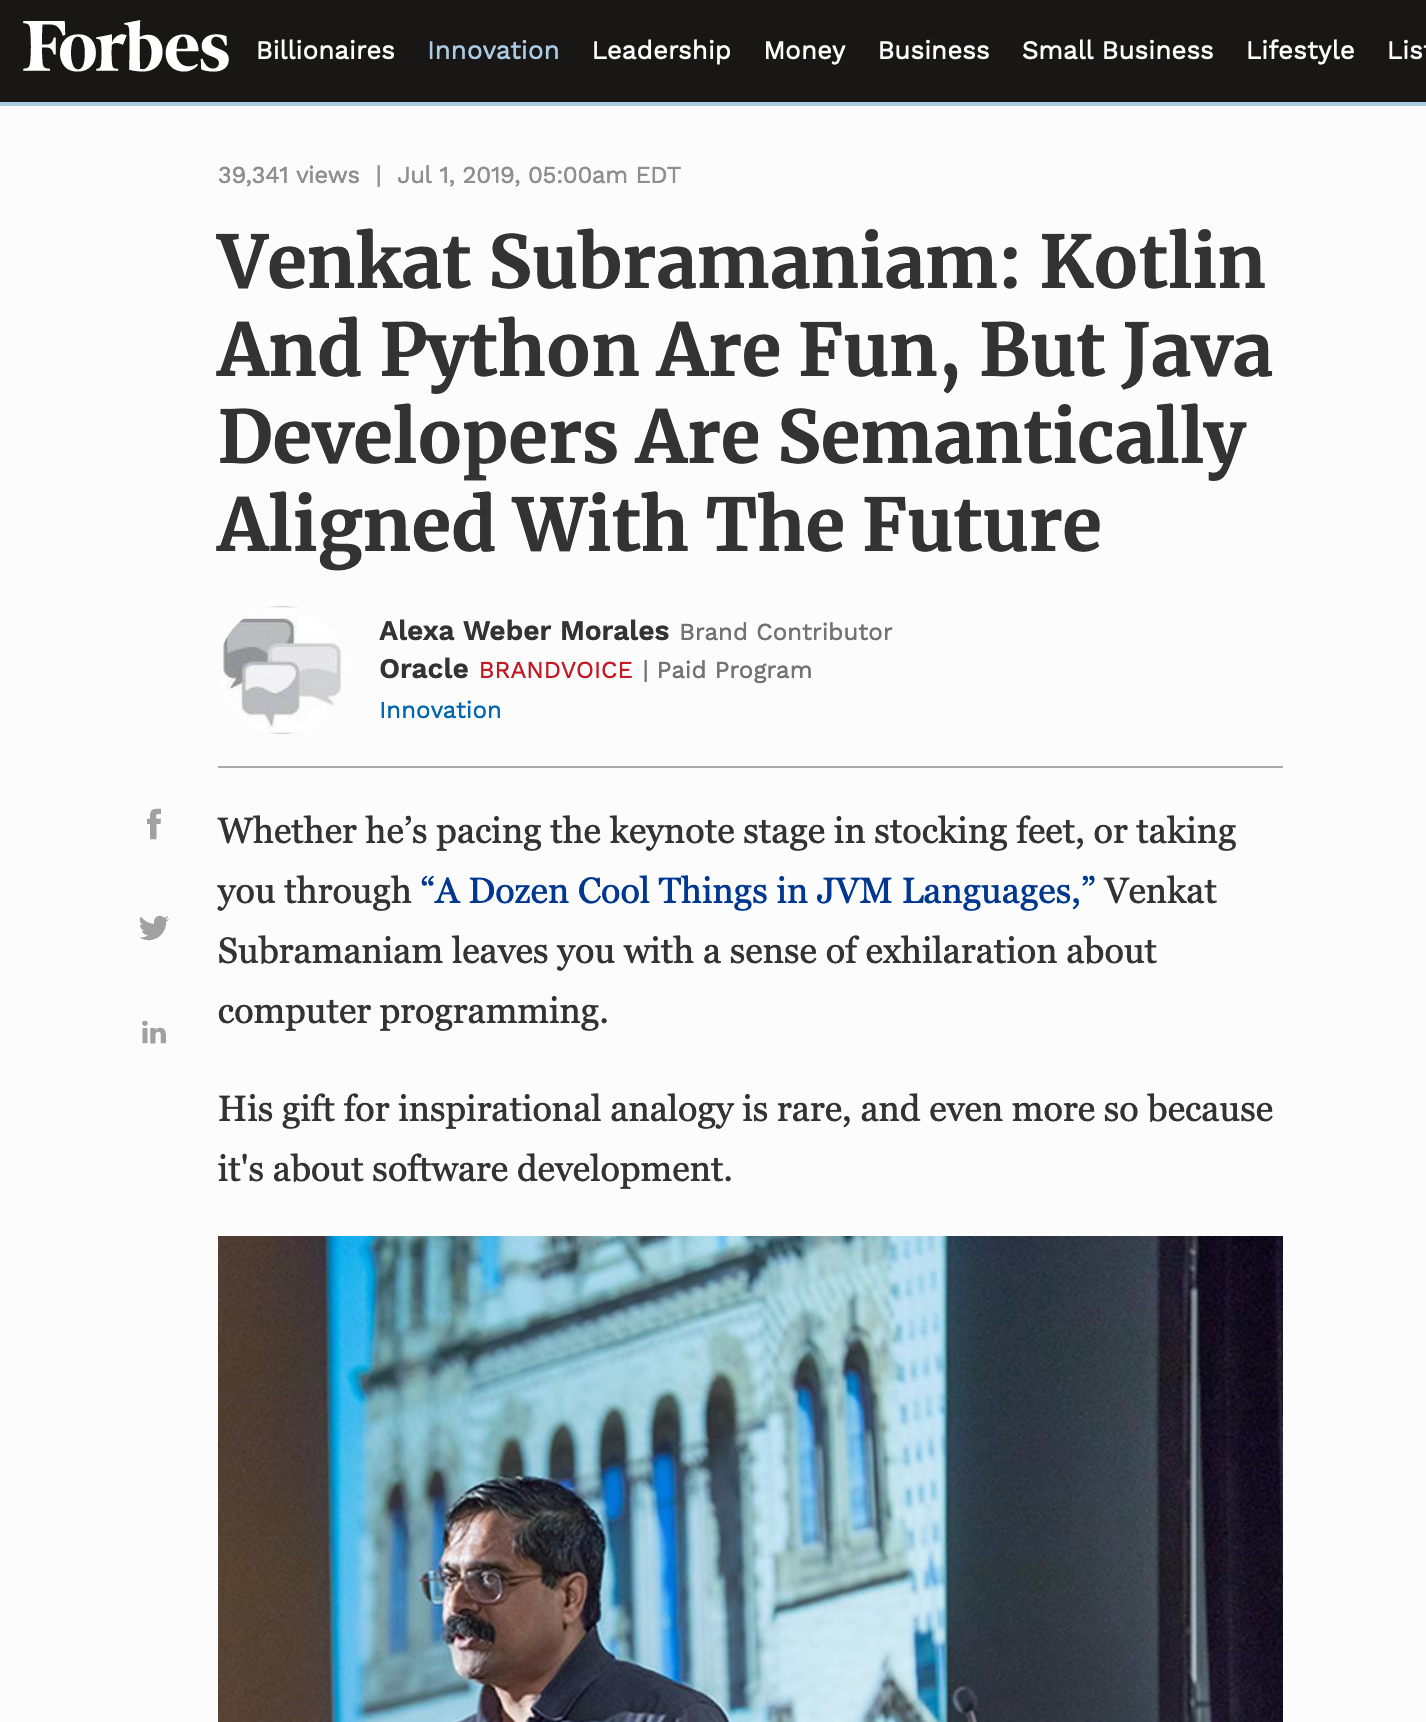
\includegraphics[width=0.5\linewidth]{Images/venkat}
    \end{figure}
\end{frame}


\section{JVM}



\begin{frame}{Lenguaje}
    ¡Yo programo en Java!
\end{frame}

\begin{frame}{Lenguaje}
    ¡Yo programo en el lenguaje Java!
\end{frame}


\begin{frame}{Lenguaje}
    ¡Yo programo en (una de) las plataformas Java!
\end{frame}


\begin{frame}{Lenguaje != Plataforma}
    \sout{Lenguaje}, Plataforma
	\begin{itemize}
	\item Compilador
    \item Entorno de ejecución
    \item APIS y bibliotecas
    \item Frameworks
    \item Editor o IDE
	\end{itemize}
\end{frame}

\begin{frame}{Lenguaje != Plataforma}
    Turbo Pascal

    \begin{columns}[T] % contents are top vertically aligned
	     \begin{column}[T]{0.5\textwidth} % each column can also be its own environment
            \begin{itemize}
                \item Compilador: Borland Pascal
                \item Bibliotecas y APIs: Borland -e.g. conio.h-
                \item Editor: Borland
            \end{itemize}
	     \end{column}
	     \begin{column}[T]{7cm} % alternative top-align that's better for graphics
   			\begin{figure}
   			\centering
   			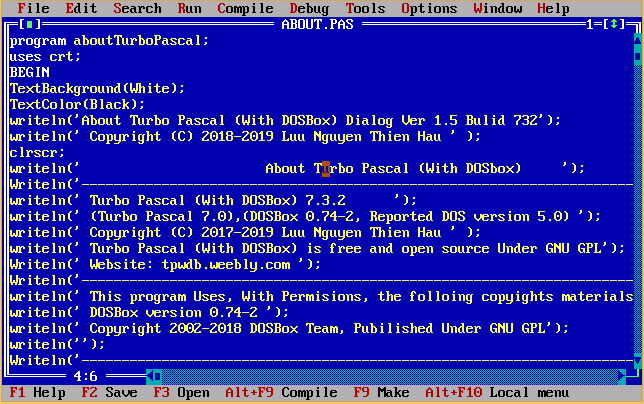
\includegraphics[width=\linewidth]{Images/pascal}
   			\end{figure}

	     \end{column}
     \end{columns}
\end{frame}

\begin{frame}{Lenguaje != Plataforma}
    Java
	\begin{itemize}
	\item Compilador: javac (OpenJDK), incremental(Eclipse JDT)
    \item Entorno ejecución: JVM -e.g. Oracle HotSpot, Amazon Correto, RedHat OpenJDK, IBM J9-, Nativo (GraalVM)
    \item Bibliotecas y APIs: OpenJDK (estandares) (Oracle, Google, RedHat), Maven Central
    \item Frameworks: Spring (VMWare), Jakarta EE (Oracle, RedHat)
    \item Editor: NetBeans (Apache), Eclipse (Eclipse), IntelliJ IDEA (JetBrains), VSCode (Microsoft)
	\end{itemize}
\end{frame}



\section{Ecosistema JVM}
\begin{frame}{JVM}
	JVM

	\begin{columns}[T] % contents are top vertically aligned
		\begin{column}[T]{0.5\textwidth} % each column can also be its own environment
			\begin{itemize}
				\item \textbf{25 años de desarrollo}
				\item Nueva versión cada 6 meses
				\item Software libre GPLv2+Classpath Exception
				\item Probablemente la maquina virtual más rápida
			\end{itemize}
		\end{column}
		\begin{column}[T]{7cm} % alternative top-align that's better for graphics
			\begin{figure}
				\centering
				
\includegraphics[width=\linewidth]{Images/openjdk}
			\end{figure}

		\end{column}
	\end{columns}
\end{frame}
\begin{frame}{}
	\begin{figure}
		\centering
		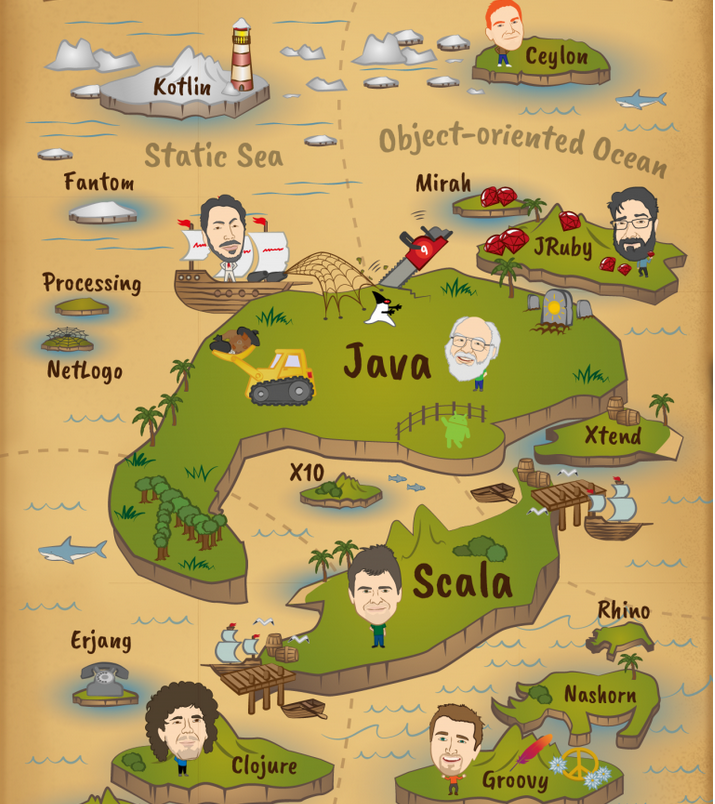
\includegraphics[width=0.5\linewidth]{Images/pirates}
	\end{figure}

\end{frame}

\begin{frame}{JVM}
	Snyk - JVM Ecosystem report 2020

	\begin{figure}
		\centering
		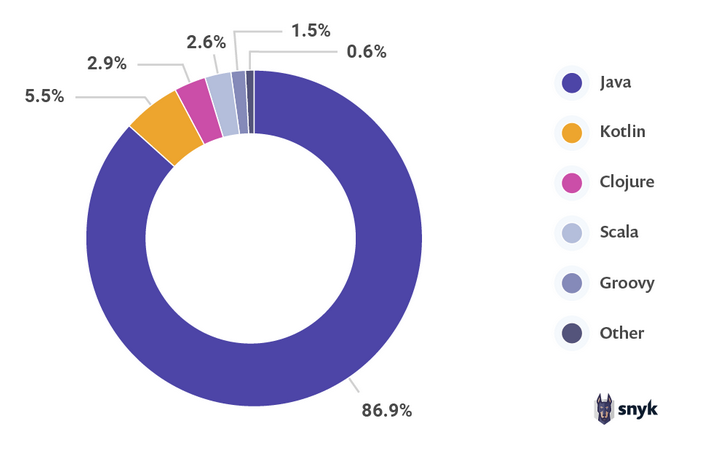
\includegraphics[width=0.7\linewidth]{Images/jvmlangs}
	\end{figure}

\end{frame}

\begin{frame}{Tendencias}
	\begin{figure}
		\centering
		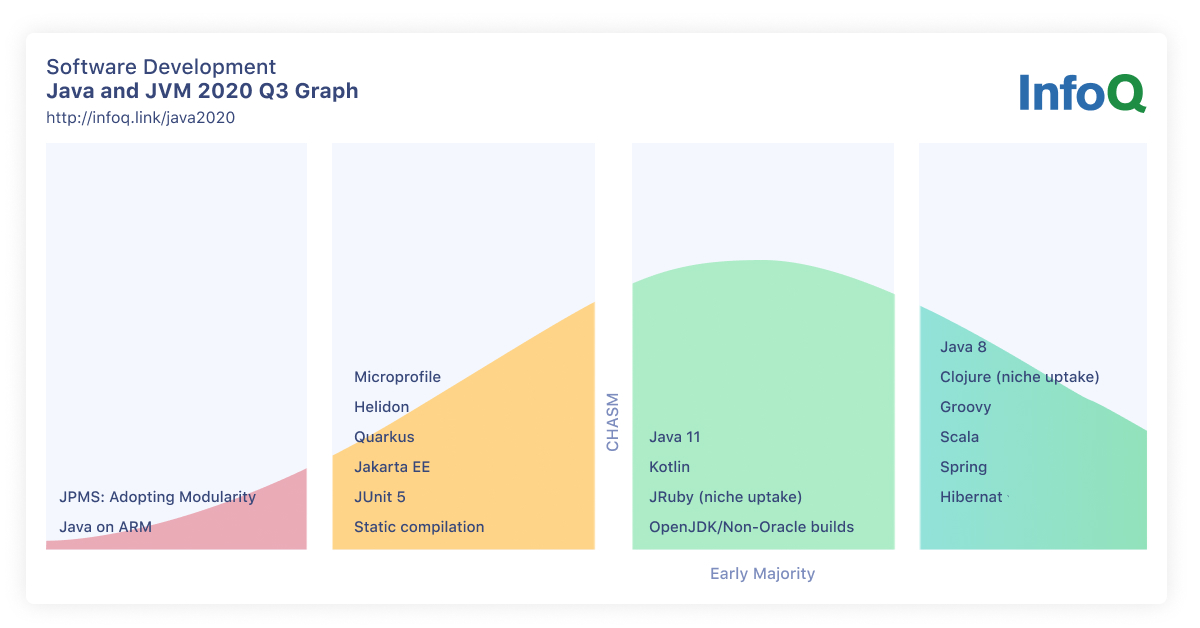
\includegraphics[width=\linewidth]{Images/trends}
	\end{figure}

\end{frame}

\begin{frame}{Distros}
jchoice.eu
	\begin{figure}
		\centering
		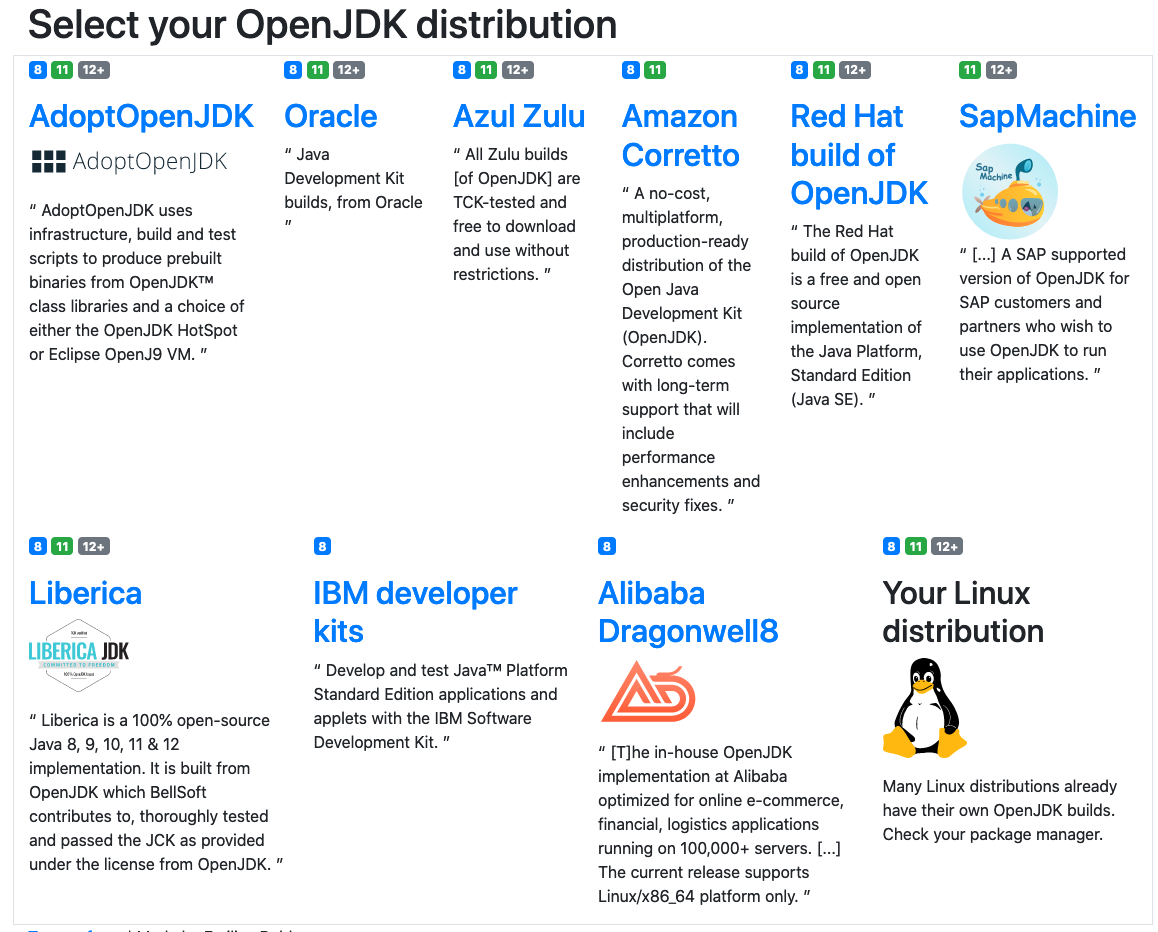
\includegraphics[width=0.7\linewidth]{Images/jdkdistros}
	\end{figure}

\end{frame}


\begin{frame}{GraalVM}

	\begin{figure}
		\centering
		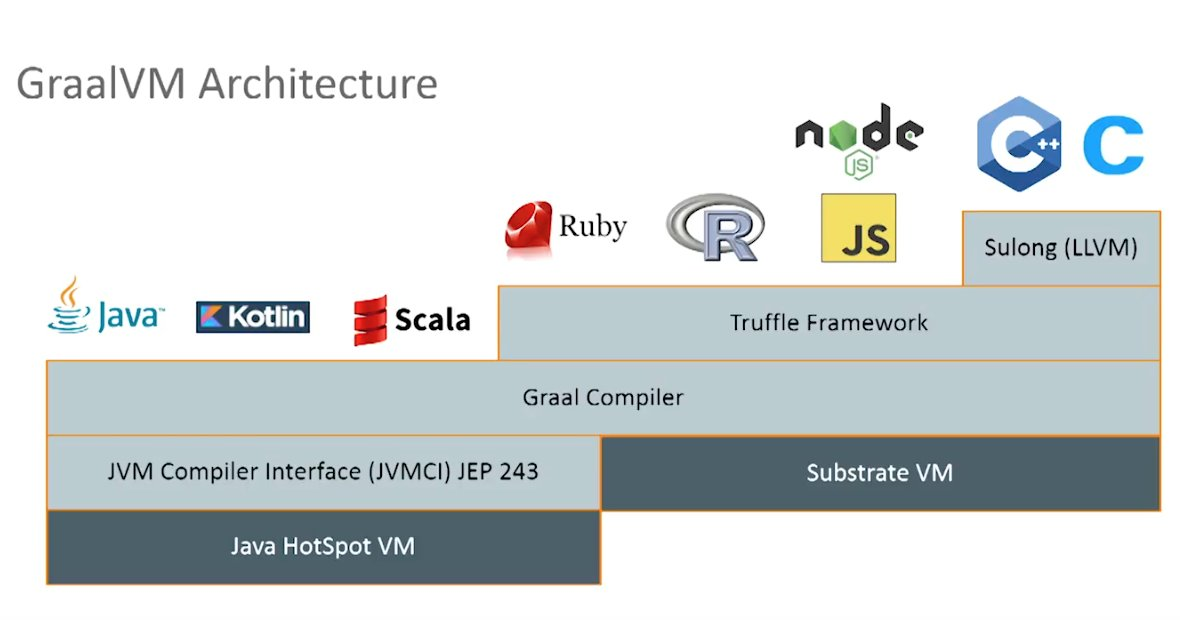
\includegraphics[width=\linewidth]{Images/graalvm}
	\end{figure}

\end{frame}

\begin{frame}{JakartaEE}

	\begin{figure}
		\centering
		
\includegraphics[width=\linewidth]{Images/jakartaee}
	\end{figure}

\end{frame}

\begin{frame}{MicroProfile}

	\begin{figure}
		\centering
		
\includegraphics[width=\linewidth]{Images/microprofile}
	\end{figure}

\end{frame}

\begin{frame}{Quarkus}

	\begin{figure}
		\centering
		
\includegraphics[width=\linewidth]{Images/quarkus}
	\end{figure}

\end{frame}


\begin{frame}{Helidon}

	\begin{figure}
		\centering
		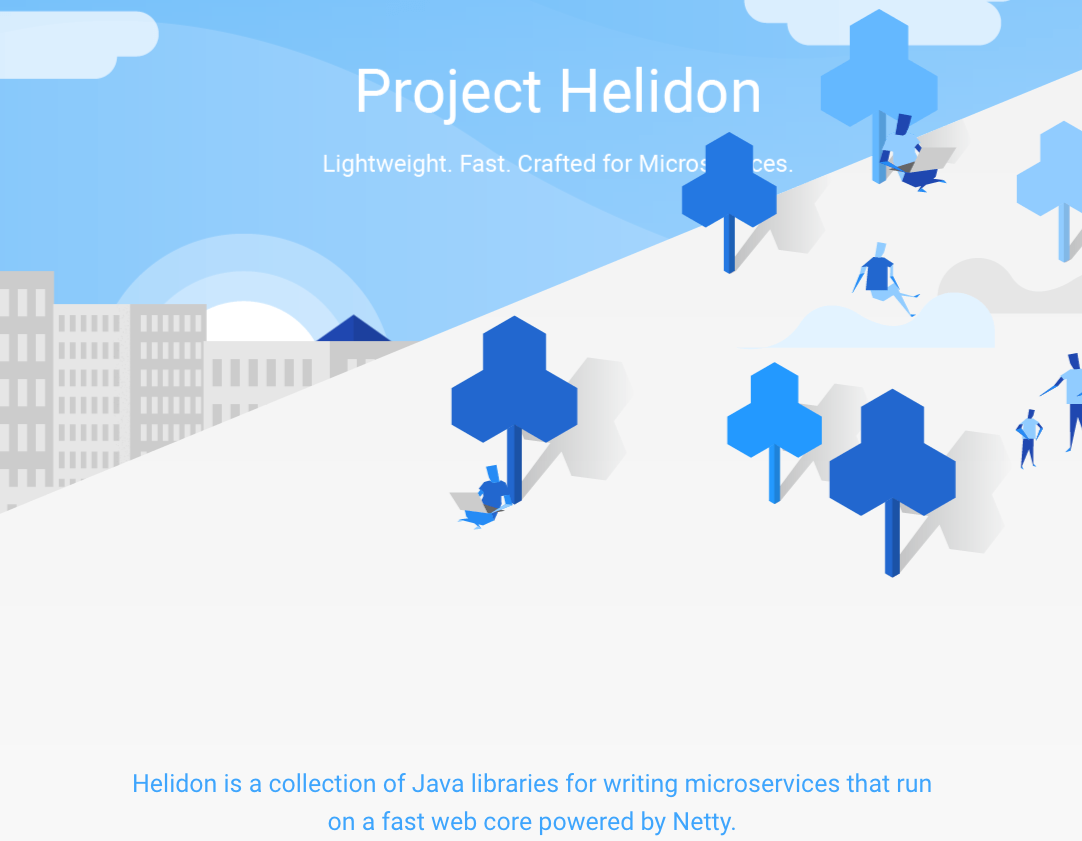
\includegraphics[width=\linewidth]{Images/helidon}
	\end{figure}

\end{frame}

\begin{frame}{Tribuo}

	\begin{figure}
		\centering
		
\includegraphics[width=\linewidth]{Images/tribuo}
	\end{figure}

\end{frame}



\begin{frame}{Víctor Orozco}
    \begin{columns}[T] % contents are top vertically aligned

        \begin{column}[T]{4cm} % alternative top-align that's better for graphics
            \begin{figure}
                \centering
                
\includegraphics[width=\linewidth]{Images/logos}
            \end{figure}
        \end{column}
        \begin{column}[T]{6cm} % each column can also be its own environment
            \begin{itemize}
                \item me@vorozco.com
                \item \href{https://twitter.com/tuxtor}{@tuxtor}
                \item \href{http://vorozco.com}{http://vorozco.com}
                \item \href{http://tuxtor.shekalug.org}{http://tuxtor.shekalug.org}
            \end{itemize}
            \begin{center}
                
\includegraphics[width=0.1\linewidth]{Images/cclogo}
                \\
                This work is licensed under Creative Commons Attribution-NonCommercial-ShareAlike 3.0 Guatemala (CC BY-NC-SA 3.0 GT).
            \end{center}
        \end{column}
    \end{columns}
\end{frame}

\end{document}

